\chapter{Contribution}

The main contribution in this thesis is to provide an active automaton learning framework, which can be used to support system design and analysis. This framework, since used in system design, is needed to be easily modifiable and extensible, while having the capability of handling any variation of formalisms systems might use.
\\\\
In order to tackle the problem of creating such a framework, I first needed to understand active automaton learning algorithms themselves.
\\
\section{Implementing a learning algorithm}

\begin{figure}
	\centering
	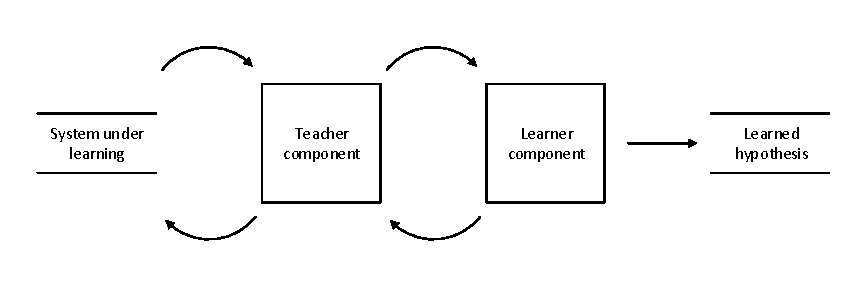
\includegraphics[width=1.0\linewidth]{figures/learningcomm}
	\caption{Data flow of active learning algorithms.}
	\label{fig:learningcomm}
\end{figure}

After processing the background knowledge seen in \cite{Steffen2011}, I decided to implement the most straightforward learning algorithm presented therein, the direct hypothesis construction algorithm.
\\
The first step was determining the formalisms used in this implementation, more specifically, the input and the output formalisms. Active automaton learning algorithms essentially have two endpoints: one being the input, reached through the teacher component, and the other being the output, where the learned hypothesis automaton is returned. This is illustrated in Fig. \ref{fig:learningcomm}. The teacher and learner component can handle abstraction, meaning the formalisms of the system under learning, or from now the input formalism, and the formalism of the learned hypothesis, or from now, the output formalism can both be arbitrary. Only implementing a specific algorithm, these formalisms needed to be specified. \\

Even if at first I was only implementing a single algorithm, the decisions on the formalism of this implementation was made with the future framework in mind. Since automaton learning algorithms can be  implemented on any type of automata, the easiest method would've been to implement DHC using deterministic finite automata. However, real-life reactive systems usually are better modeled using Mealy machines, hence the implementation was made using Mealy machines as both input and output formalisms.
\\
The first step of the implementation process was choosing the right tooling. This decision was also formed by the future system design perspective, which is why the Mealy machine implementation was done in Eclipse Modeling Framework.
\\\\
Eclipse Modeling Framework (EMF), or more specifically, EMF core, is an "abstraction for describing, composing, and manipulating structured information", essentially a tool for system modeling and code generation implemented in Java. Figure \ref*{fig:mealyecore} shows an UML class diagram of the metamodel I've created using the Ecore package of EMF core. 

\begin{figure}
	\centering
	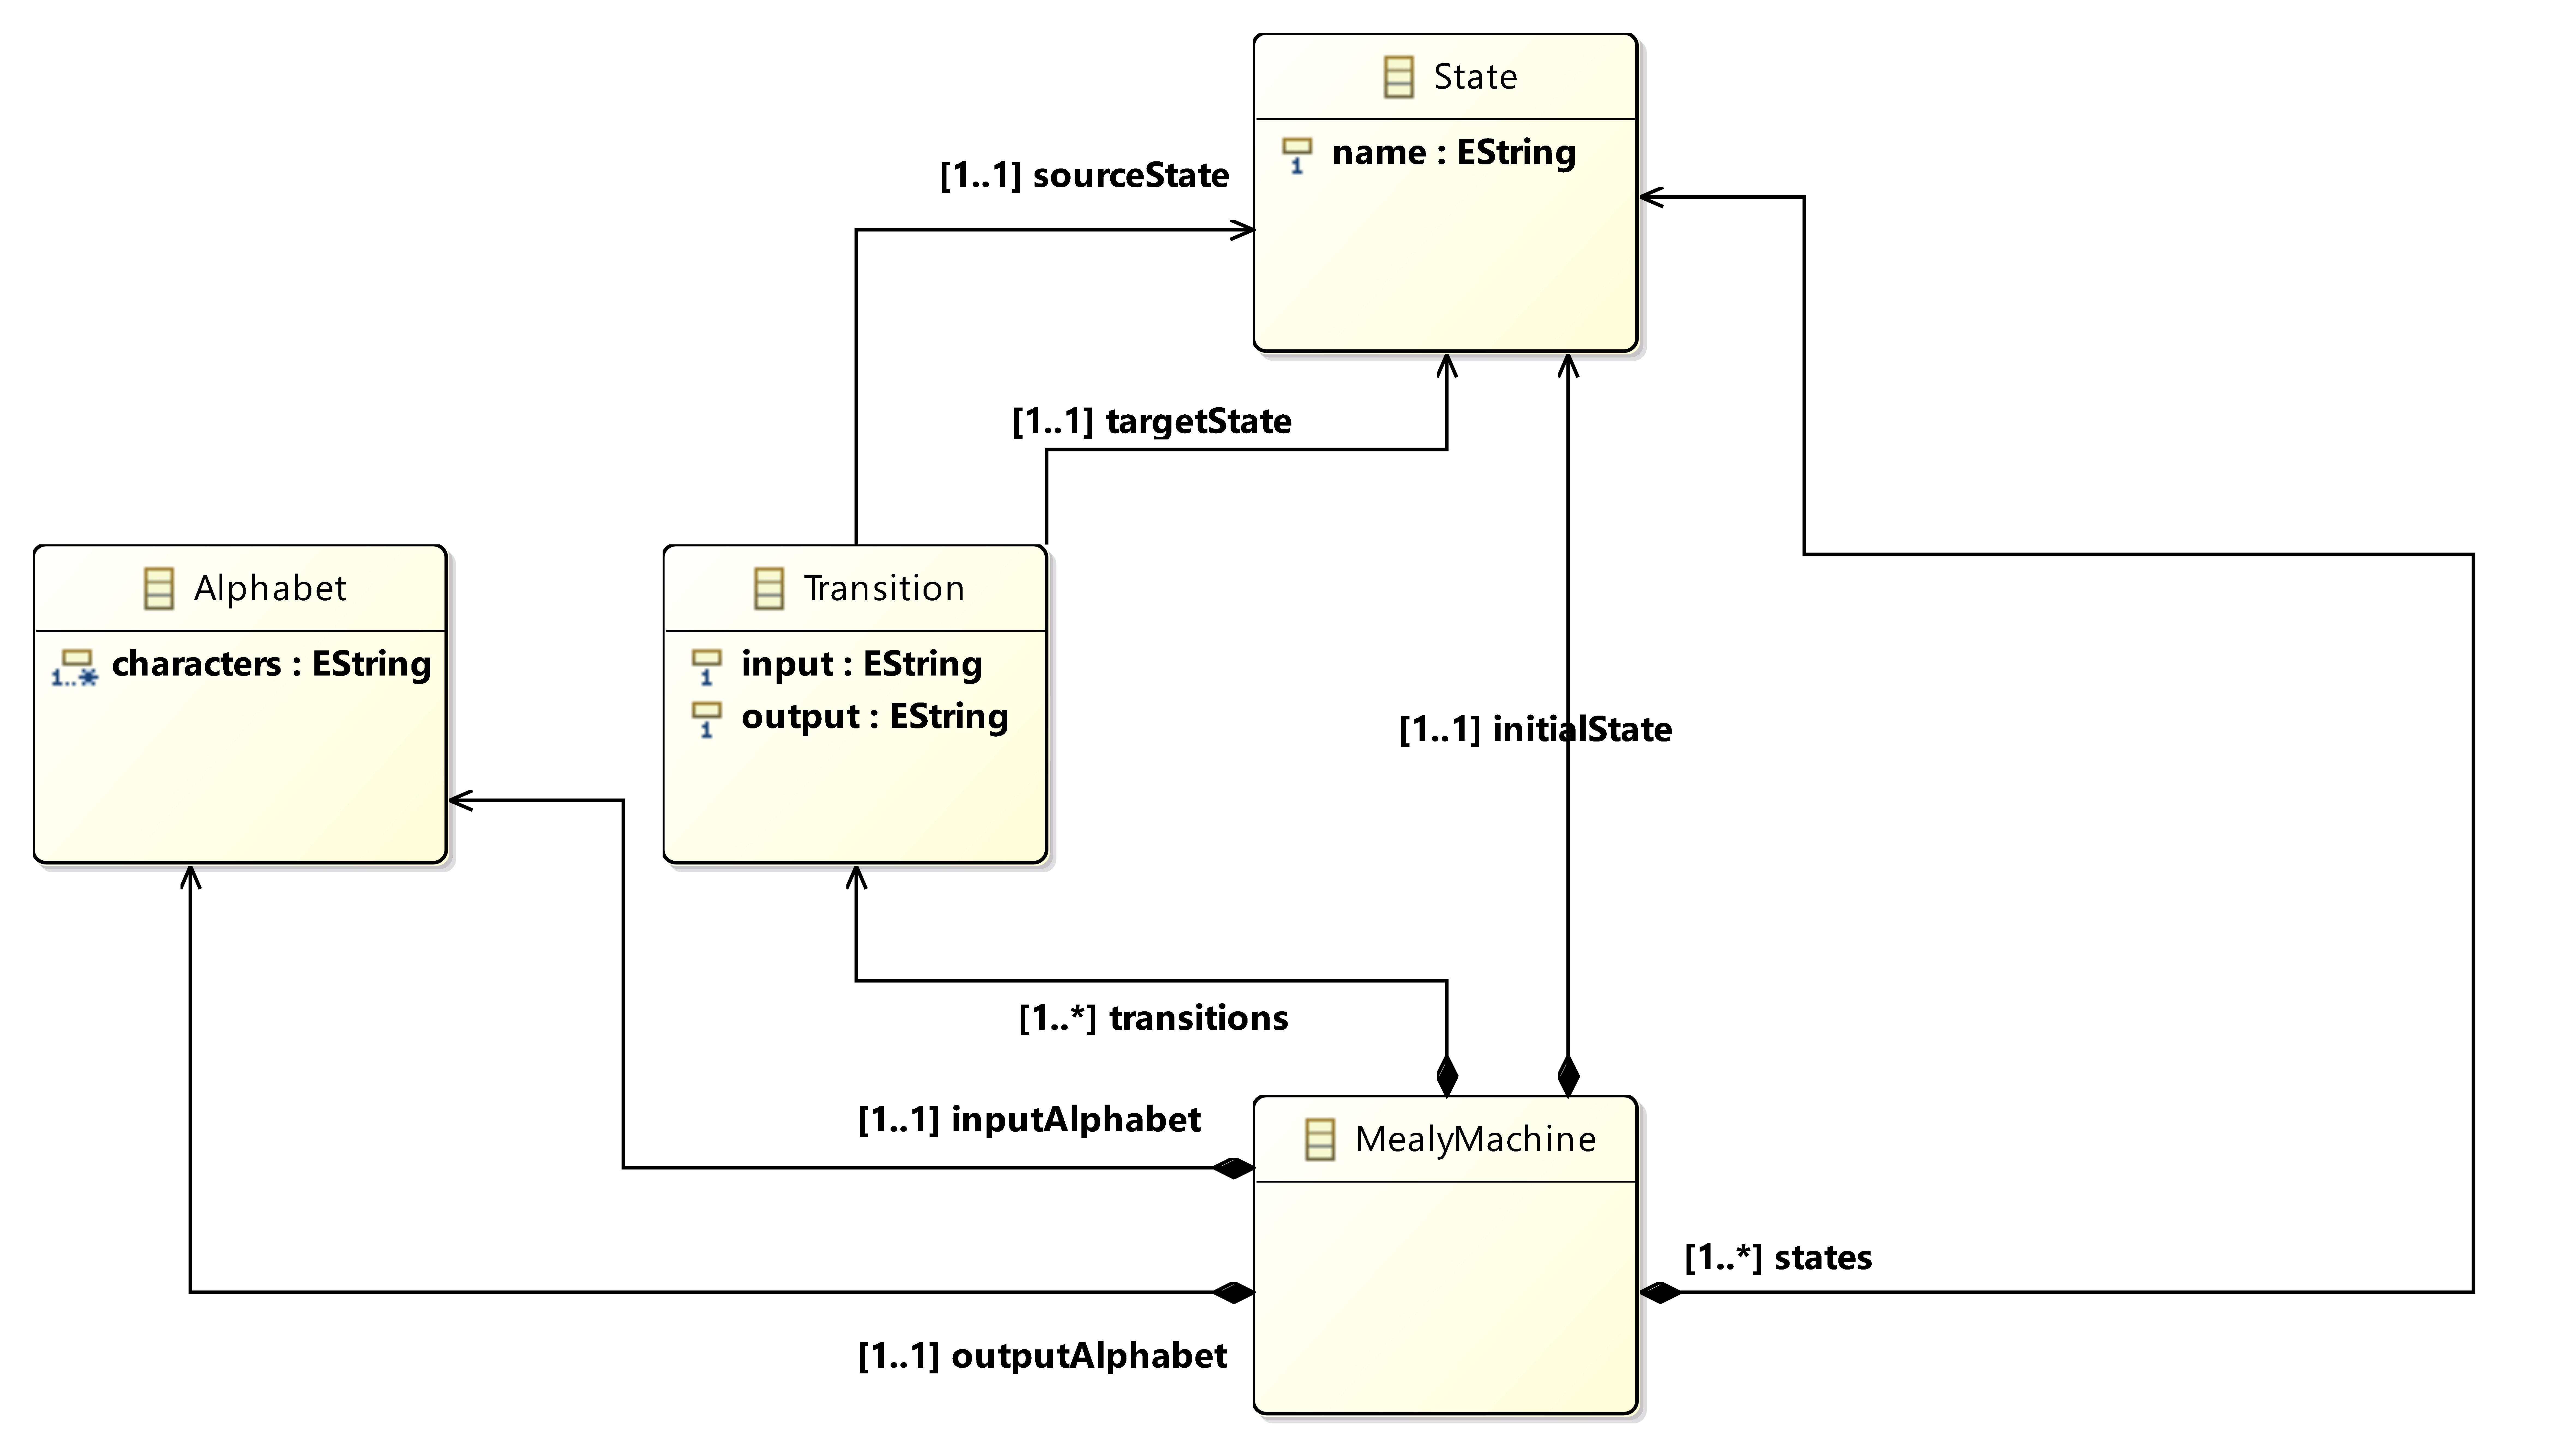
\includegraphics[width=1.0\linewidth]{figures/mealymodel}
	\caption{Ecore metamodel of Mealy machines.}
	\label{fig:mealyecore}
\end{figure}

In text, the Ecore model I've created uses Strings as distinguishers (on code generation, EString is converted to java.lang.String). States of the automaton, i.e. State objects are differentiated based on the name field. Note, that this is a transition-driven model of mealy machines, the Transition class stores the source and target states of the transition, as opposed to some models, where states store their own transition information (successors, predecessors) like nodes in a graph. This decision was based on the DHC algorithm, which while learning, stores traversal information itself, rather than asking for it, which is why ease of access is preferred as opposed to efficiency.
\\\\
Using EMF, I generated the class diagram seen in Fig. \ref{fig:mealyecore} into Java code. With this code, I implemented the direct hypothesis construction algorithm (in Java as well), without any framework whatsoever, only a single class accepting a MealyMachine object and constructing a Hypothesis MealyMachine object based off of it. In order to run and test this implementation, an example was needed, for which I chose the automaton seen in \ref{fig:coffeemealy}. Programmatically creating this example as an object is not a scalable solution, espetially regarding the future framework to be built, so I used Xtext, another tool, to solve this issue.
\\
Xtext is a framework for creating programming and domain-specific languages, which also has integration with EMF metamodels. Using this integration, I generated the Xtext grammar seen in Listing \ref{li:xtext}. In words, this  grammar describes a textual grammar in which instances of the metamodel seen in Fig. \ref{fig:mealyecore} can be stored. 



\begin{lstlisting}[caption=Xtext grammar describing Mealy machines.,label=li:xtext]
MealyMachine returns MealyMachine:
	'MealyMachine'
	'{'
		'initialState' initialState=State
		'states' '{' states+=State ( "," states+=State)* '}' 
		'inputAlphabet' inputAlphabet=Alphabet
		'outputAlphabet' outputAlphabet=Alphabet
		'transitions' '{' transitions+=Transition ( "," transitions+=Transition)* '}' 
	'}';
	
State returns State:
	{State}
	'State'
	name=EString;

Alphabet returns Alphabet:
	'Alphabet'
	'{'
		'characters' '{' characters+=EString ( "," characters+=EString)* '}' 
	'}';

Transition returns Transition:
	'Transition'
	'{'
		'input' input=EString
		'output' output=EString
		'sourceState' sourceState=[State|EString]
		'targetState' targetState=[State|EString]
	'}';

EString returns ecore::EString:
STRING | ID;
\end{lstlisting}

Utilizing the Xtext grammar in Listing \ref{li:xtext}, I created the input to be used by the implemented DHC, containing the formalized version of the automaton shown in Fig. \ref{fig:coffeemealy}. The input file can bee seen in Listing \ref{li:coffeemealy}


\begin{lstlisting}[caption=The Mealy machine seen in Fig.\ref{fig:coffeemealy} in the form of the Xtext the grammar described in Listing \ref{li:xtext}.,label=li:coffeemealy]
	MealyMachine{
		initialState 
		State a states { State a, State b, State c, State d, State e, State dd, State f
		}inputAlphabet Alphabet { characters { water , pod , button , clean } }
		outputAlphabet Alphabet { characters { done , coffee , none } }
		transitions{ 
		Transition { input clean output done sourceState a targetState a } , 
		Transition { input pod output done sourceState a targetState b } , 
		Transition { input water output done sourceState a targetState c } , 
		Transition { input button output none sourceState a targetState f } , 
		Transition { input pod output done sourceState b targetState b } , 
		Transition { input water output done sourceState b targetState d } , 
		Transition { input button output none sourceState b targetState f } , 
		Transition { input clean output done sourceState b targetState a } , 
		Transition { input clean output done sourceState c targetState a } , 
		Transition { input pod output done sourceState c targetState dd } , 
		Transition { input button output none sourceState c targetState f } , 
		Transition { input water output done sourceState c targetState c } , 
		Transition { input water output done sourceState d targetState d } , 
		Transition { input pod output done sourceState d targetState d } , 
		Transition { input clean output done sourceState d targetState a } , 
		Transition { input button output coffee sourceState d targetState e } , 
		Transition { input water output done sourceState dd targetState dd } , 
		Transition { input pod output done sourceState dd targetState dd } , 
		Transition { input button output coffee sourceState dd targetState e } , 
		Transition { input clean output done sourceState dd targetState a } , 
		Transition { input clean output done sourceState e targetState a } , 
		Transition { input button output none sourceState e targetState f } , 
		Transition { input pod output none sourceState e targetState f } , 
		Transition { input water output none sourceState e targetState f } , 
		Transition { input clean output none sourceState f targetState f } , 
		Transition { input button output none sourceState f targetState f } , 
		Transition { input pod output none sourceState f targetState f } , 
		Transition { input water output none sourceState f targetState f } } }
\end{lstlisting}